\documentclass[12pt,a4paper]{article}

% ====== PAQUETES BÁSICOS ======
\usepackage[spanish]{babel}
\usepackage[utf8]{inputenc}
\usepackage[T1]{fontenc}
\usepackage{graphicx}
\usepackage{float}
\usepackage{amsmath, amssymb}
\usepackage{booktabs}
\usepackage{hyperref}
\usepackage{geometry}
\geometry{margin=2.5cm}
\usepackage{caption}
\usepackage{fancyhdr}

% --- para envolver texto en tablas y permitir cortes dentro de \texttt
\usepackage{tabularx}
\usepackage{array}
\usepackage{ragged2e}   % para \RaggedRight que sí permite cortes
\usepackage{seqsplit}   % corta tokens largos en cualquier punto seguro
\usepackage{microtype}  % mejora espaciado (opcional)

\newcolumntype{Y}{>{\RaggedRight\arraybackslash}X}  % columna expandible con saltos
\newcolumntype{L}[1]{>{\RaggedRight\arraybackslash}p{#1}} % ancho fijo con saltos

% Macro para código que sí puede partir en líneas
\newcommand{\code}[1]{\texttt{\seqsplit{#1}}}

% Opcional: un pelín menos de padding y algo más de alto de fila
\setlength{\tabcolsep}{6pt}
\renewcommand{\arraystretch}{1.12}

% ====== CONFIGURACIÓN DE ENCABEZADO ======
\pagestyle{fancy}
\fancyhf{}
\lhead{TD VI – Inteligencia Artificial}
\rhead{TP2 – Spotify Forward Prediction}
\cfoot{\thepage}

% ====== DATOS DE PORTADA ======
\title{\vspace{-2cm}\textbf{Trabajo Práctico 2: Tecnología Digital VI}\\[0.2cm]
\large Predicción de presionar “Forward” en Spotify}
\author{Facundo Amaya \and Juan Ignacio Elosegui \and Nicolás Boudourian}
\date{Universidad Torcuato Di Tella \\ Segundo cuatrimestre 2025}

\begin{document}

\maketitle
\thispagestyle{empty}
\vspace{1cm}

\begin{abstract}
\noindent
En este trabajo se desarrolla un sistema de aprendizaje automático para predecir si un usuario presionará el botón \textit{forward} en una canción de Spotify, a partir de información de sesiones de escucha. 
Se presentan las etapas de análisis exploratorio, creación de variables, estrategia de validación, modelado y análisis de importancia de atributos.
\end{abstract}

\newpage

% ==============================================================
\section{Introducción}

En este trabajo se desarrolló un sistema de aprendizaje automático para predecir si un usuario de Spotify presionará el botón \textit{forward} durante la reproducción de una canción. 
El problema se aborda como una tarea de clasificación binaria, donde la variable objetivo toma el valor $1$ cuando \texttt{reason\_end = "fwdbtn"} y $0$ en caso contrario.  

La métrica de evaluación utilizada es el \textbf{ROC-AUC}, dado que mide la capacidad discriminativa del modelo independientemente del umbral de decisión.  
El enfoque adoptado combina ingeniería de variables temporales y de comportamiento del usuario, validación temporal y un modelo basado en \textbf{XGBoost}, un algoritmo de gradient boosting sobre árboles de decisión.

% ==============================================================

\section{Análisis Exploratorio de Datos (EDA)}

El dataset original provisto por la competencia se encuentra dividido en dos archivos: 
\begin{itemize}
    \item \texttt{train\_data.txt}: contiene observaciones históricas con la variable \texttt{reason\_end}.
    \item \texttt{test\_data.txt}: idéntico formato pero sin la columna \texttt{reason\_end}.
\end{itemize}

Cada fila representa una reproducción de una canción por un usuario identificado por \texttt{username}, con información asociada como hora, país de conexión, plataforma y metadatos de la canción.  

Durante el análisis exploratorio se detectaron:
\begin{itemize}
    \item Variables categóricas de alta cardinalidad (\texttt{master\_metadata\_track\_name}, \texttt{master\_metadata\_album\_artist\_name}, etc.).
    \item Campos booleanos (\texttt{shuffle}, \texttt{offline}, \texttt{incognito\_mode}).
    \item Campos temporales (\texttt{ts}, \texttt{offline\_timestamp}) a partir de los cuales se construyeron patrones temporales.
\end{itemize}

\noindent \textbf{Patrones relevantes observados:}
\begin{itemize}
    \item Mayor frecuencia de \textit{forward} en los primeros temas de una sesión.
    \item Comportamiento diferenciado entre fines de semana y días hábiles.
    \item Usuarios con historial previo de saltos tienden a repetir ese comportamiento.
\end{itemize}

Además, encontramos otros dos patrones:
\begin{figure}[H]
    \centering
    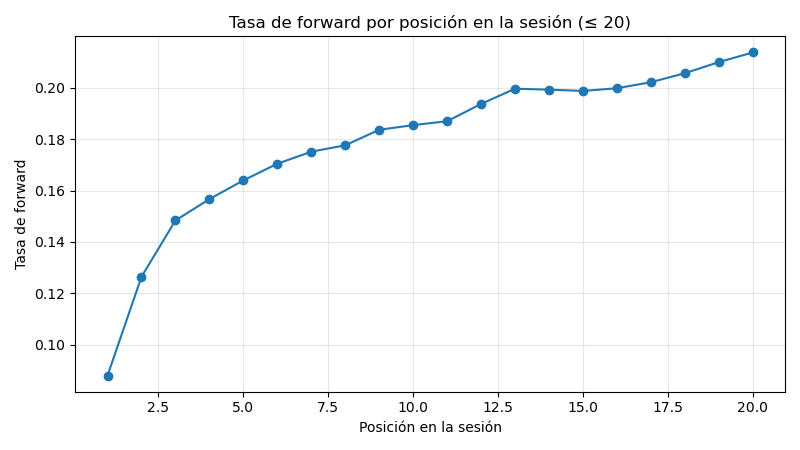
\includegraphics[width=0.8\linewidth]{fig1.png}
    \caption{Tasa de forward por posición en la sesión.}
\end{figure}
La tasa de forward (probabilidad de que el usuario salte la canción) aumenta a medida que avanza la sesión.
Al principio (posición 1–3) los usuarios escuchan más tiempo y saltan menos, pero después de varios temas la probabilidad de salto se incrementa progresivamente, alcanzando un ~21\% en la posición 20. \\
Al comienzo de una sesión el usuario suele estar más activo eligiendo música que le gusta o ajustando la lista; más adelante, puede distraerse, cansarse o buscar variedad, lo que genera más saltos. También puede reflejar que las canciones al inicio son de mayor preferencia o que el modelo de recomendación las ordena según relevancia.

\begin{figure}[H]
    \centering
    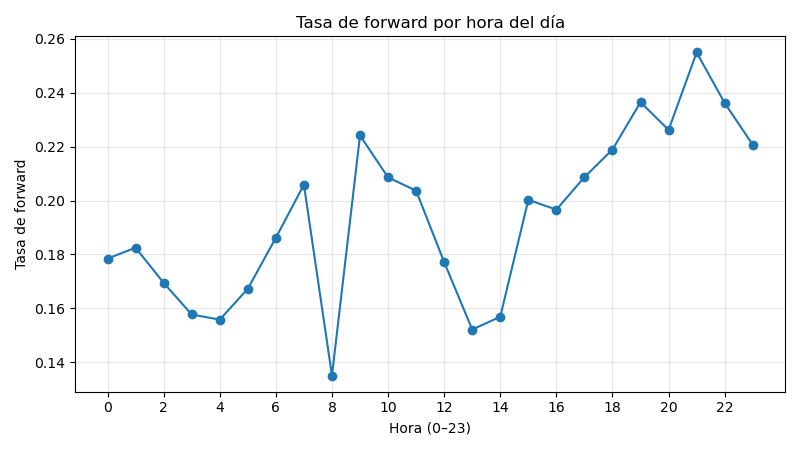
\includegraphics[width=0.8\linewidth]{fig2.png}
    \caption{Tasa de forward por hora del día.}
\end{figure}
Se observan fluctuaciones horarias: menor tasa de saltos entre las 3 y las 6 h, picos cerca de las 10 h y entre las 19–22 h. Las horas nocturnas y de noche presentan más saltos, mientras que la madrugada y el mediodía son más estables o con tasas más bajas.\\
Durante la mañana o el trabajo, los usuarios suelen dejar la música de fondo y saltan menos. En cambio, al final del día (tarde/noche), escuchan más activamente y seleccionan canciones, generando más forwards. Los picos de la noche pueden coincidir con ocio o actividad social.

% ==============================================================

\section{Creación de Variables}

Se implementó un proceso de \textbf{feature engineering} que combina información temporal, de usuario y de artista.  
Las principales variables creadas fueron:

\begin{table}[H]
    \centering
    \small
    \caption{Principales variables derivadas en el pipeline.}
    \begin{tabularx}{\textwidth}{@{} L{3.4cm} L{3.1cm} Y @{}}
        \toprule
        \textbf{Variable} & \textbf{Fuente} & \textbf{Descripción} \\
        \midrule
        \code{hour}, \code{dow} & \code{ts} & Hora y día de la semana de reproducción \\
        \code{hour\_sin}, \code{hour\_cos}, \code{dow\_sin}, \code{dow\_cos} & \code{ts} & Representación cíclica de hora y día \\
        \code{secs\_since\_prev} & Diferencia entre reproducciones & Segundos desde la última reproducción del mismo usuario \\
        \code{log1p\_secs\_since\_prev} & \code{secs\_since\_prev} & Escala logarítmica para valores extremos \\
        \code{user\_forward\_rate\_hist} & Historial usuario & Promedio histórico de forwards (suavizado bayesiano) \\
        \code{user\_roll\_mean \{3,5,10\}} & Historial reciente & Promedio móvil de los últimos 3, 5 y 10 eventos \\
        \code{secs\_since\_last\_forward} & Eventos previos & Tiempo desde el último \textit{forward} \\
        \code{user\_artist\_rate\_hist} & user–artist & Probabilidad histórica de forward para un artista específico \\
        \code{artist\_freq} & Entrenamiento & Frecuencia global del artista (popularidad) \\
        \code{session\_id}, \code{pos\_in\_session} & \code{ts} & Segmentación en sesiones (gaps $>$ 30 min) y posición dentro de la sesión \\
        \code{is\_first\_in\_session} & \code{pos\_in\_session} & Indicador de primer tema en la sesión \\
        \bottomrule
    \end{tabularx}
\end{table}

También se aplicaron transformaciones trigonométricas para capturar periodicidad diaria y semanal, y codificación categórica mediante \texttt{OneHotEncoder} dentro de un \texttt{ColumnTransformer}.

% ==============================================================

\section{Construcción del Conjunto de Validación}

Dado que el comportamiento de los usuarios y la secuencia temporal son relevantes, se optó por un \textbf{split temporal} para validación.  
Se utilizó el 90\% inicial de las observaciones (ordenadas por \texttt{ts}) para entrenamiento y el 10\% más reciente para validación:

\[ \text{train: } t < q_{0.9}(\text{ts}) \quad ; \quad \text{valid: } t \ge q_{0.9}(\text{ts}) \]

Este esquema evita fuga temporal (\textit{data leakage}) entre entrenamiento y validación, y emula la dinámica real de predicción sobre sesiones futuras.

% ==============================================================

\section{Modelos y Búsqueda de Hiperparámetros}

El modelo final utilizado fue un \textbf{XGBoost Classifier} con las siguientes configuraciones principales:

\begin{table}[H]
\centering
\begin{tabular}{ll}
\toprule
\textbf{Parámetro} & \textbf{Valor} \\
\midrule
n\_estimators & 3000 \\
learning\_rate & 0.03 \\
max\_depth & 4 \\
min\_child\_weight & 4 \\
subsample, colsample\_bytree & 0.9 \\
reg\_lambda, reg\_alpha & 1.0, 0.1 \\
early\_stopping\_rounds & 100 \\
tree\_method & hist \\
\bottomrule
\end{tabular}
\caption{Configuración de hiperparámetros del modelo XGBoost.}
\end{table}

Se evaluaron distintos modelos de clasificación (árboles de decisión, regresión logística y métodos de boosting). 
Seleccionamos \textbf{XGBoost} finalmente por su excelente desempeño en tareas con datos tabulares heterogéneos, por su capacidad para manejar relaciones no lineales y variables con distintas escalas, y por contar con regularización interna que reduce el riesgo de sobreajuste. 
Además, ofrece alta eficiencia computacional gracias a su implementación paralelizada y soporte para \textit{early stopping}, lo que permite ajustar los hiperparámetros de manera precisa y rápida.

Se aplicó \textbf{early stopping} monitoreando el AUC en el conjunto de validación temporal.  
El modelo se entrenó con una ponderación inversa de clases (\texttt{scale\_pos\_weight}) para compensar el desbalance entre eventos de forward y no-forward.

El resultado de validación obtenido fue aproximadamente:
\[ \text{AUC}_{valid} \approx 0.78 \]

El conjunto de test se transformó con el mismo preprocesador y se generó un archivo \texttt{modelo\_xgb.csv} con las probabilidades predichas de \textit{forward}.

% ==============================================================

\section{Importancia de Atributos}

El análisis de importancia de variables (\textit{feature importance}) reveló que los predictores más influyentes son los relacionados al historial del usuario y su comportamiento temporal:

\begin{itemize}
    \item \texttt{user\_forward\_rate\_hist}: predictor dominante, refleja la propensión del usuario a saltar canciones.
    \item \texttt{secs\_since\_prev}: tiempos largos entre reproducciones reducen la probabilidad de forward.
    \item \texttt{pos\_in\_session}: los primeros temas presentan mayor probabilidad de salto.
    \item \texttt{user\_artist\_rate\_hist}: mide la afinidad usuario–artista.
    \item \texttt{hour\_sin} / \texttt{hour\_cos}: reflejan patrones horarios de escucha.
\end{itemize}

En general, las variables temporales y de historial del usuario aportaron más información que las categóricas (\texttt{platform}, \texttt{conn\_country}, etc.).

% ==============================================================

\section{Conclusiones}

El sistema propuesto alcanza un desempeño sólido (AUC $\approx 0.78$) utilizando un pipeline reproducible y eficiente basado en XGBoost.  
Las claves del buen rendimiento fueron:
\begin{itemize}
    \item Un \textbf{feature engineering} centrado en comportamiento temporal y usuario–artista.
    \item Un \textbf{esquema de validación temporal} que evita fugas de información.
    \item Un \textbf{modelo robusto y rápido}, con \textit{early stopping} y regularización moderada.
\end{itemize}

\noindent \textbf{Limitaciones:}
\begin{itemize}
    \item No se incorporaron embeddings ni variables de audio de la API de Spotify.
\end{itemize}

\noindent \textbf{Futuras mejoras:}
\begin{itemize}
    \item Integrar información externa (popularidad, duración, audio features).

\end{itemize}

% ==============================================================

\section*{Referencias}
\begin{itemize}
    \item Kaggle Competition: \url{https://www.kaggle.com/t/1ec753ebddb246ee86e6731ec097c6e1}
    \item Spotify API Documentation: \url{https://developer.spotify.com/documentation/web-api}
\end{itemize}

\end{document}
